\subsection{Introduction}

The design is based in the following assumptions:

\begin{itemize}
\item Design wall with pinned base and pinned top.
\item Neglect corner regions (wall spans one-way only).
\item Top slab is in place and has achieved full strength prior to back-filling.
\item Vehicular traffic around the building is represented by a uniform load of $250\ psf$ ($11.97\ kN/m^2$).
\item The vertical response of the soil calculated using a Winkler model with a sub-grade reaction module of set of 200 pounds per cubic inch ($54.29 \times 10^6\ N/m^3$).
\item Water table deep below structure.
\end{itemize}

\subsection{Load determination}

\subsubsection{Self weight}
The self weight of the reinforced concrete is calculated from its density: $2500\ kg/m^3$.

\subsubsection{Axial loads from building}
The loads transferred by the top slab to the wall are as follows:

\begin{center}
  \begin{tabular}{|l|l|r|r|}
\hline
\textbf{Building} & \textbf{Load} & \textbf{Phase 1} & \textbf{Phase 2}\\
\textbf{side} &  & (kN/m) & (kN/m)\\
\hline
North & SnowL & 10.06 & 10.06\\
North & LiveL & 21.67 & 21.67\\
North & Wind\_NS & -15.12 & -15.12\\
North & Wind\_WE & -1.33 & -1.33\\
North & DeadL & 31.54 & 31.54\\
\hline
South & SnowL & 8.04 & 16.08\\
South & LiveL & 14.22 & 28.44\\
South & Wind\_NS & 4.97 & 9.95\\
South & Wind\_WE & -0.23 & -0.46\\
South & DeadL & 20.58 & 41.15\\
\hline
East & SnowL & 11.96 & 11.96\\
East & LiveL & 23.75 & 23.75\\
East & Wind\_NS & -0.07 & -0.07\\
East & Wind\_WE & 12.97 & 12.97\\
East & DeadL & 30.87 & 30.87\\
\hline
West & SnowL & 15.02 & 15.02\\
West & LiveL & 27.15 & 27.15\\
West & Wind\_NS & -0.20 & -0.20\\
West & Wind\_WE & -13.20 & -13.20\\
West & DeadL & 29.81 & 29.81\\
\hline
\end{tabular}
\end{center}

\subsection{Load combinations}

\begin{center}
  \begin{footnotesize}
  \begin{tabular}{|l|c|l|}
\hline
\multicolumn{3}{|c|}{\textbf{Serviceability limit states}}\\
\hline
Equation 16-8 & EQ1608 & 1.0*selfWeight+1.0*deadLoad\\
Equation 16-9 & EQ1609A & 1.0*selfWeight+1.0*deadLoad+1.0*trafficLoad\\
Equation 16-9 & EQ1609B & 1.0*selfWeight+1.0*deadLoad+1.0*liveLoad\\
Equation 16-10 & EQ1610 & 1.0*selfWeight+1.0*deadLoad+1.0*snowLoad\\
Equation 16-11 & EQ1611A & 1.0*selfWeight+1.0*deadLoad+0.75*trafficLoad+0.75*snowLoad\\
Equation 16-11 & EQ1611B & 1.0*selfWeight+1.0*deadLoad+0.75*liveLoad+0.75*snowLoad\\
Equation 16-12 & EQ1612 & 1.0*selfWeight+1.0*deadLoad+0.6*windLoad\\
Equation 16-13 & EQ1613A & 1.0*selfWeight+1.0*deadLoad+0.45*windLoad+0.75*trafficLoad+0.75*snowLoad\\
Equation 16-13 & EQ1613B & 1.0*selfWeight+1.0*deadLoad+0.45*windLoad+0.75*liveLoad+0.75*snowLoad\\
Equation 16-14 & \multicolumn{2}{l|}{doesn't apply}\\
Equation 16-15 & EQ1615 & 0.6*selfWeight+0.6*deadLoad+0.6*windLoad\\
Equation 16-16 & \multicolumn{2}{l|}{doesn't apply}\\
\hline
  \end{tabular}
  \end{footnotesize}
  \end{center}


\begin{center}
  \begin{footnotesize}
  \begin{tabular}{|l|c|l|}
\hline
\multicolumn{3}{|c|}{\textbf{Ultimate limit states.}}\\
\hline
Equation 16-1 & EQ1601 & 1.4*selfWeight+1.4*deadLoad\\
Equation 16-2 & EQ1602A & 1.2*selfWeight+1.2*deadLoad+1.6*trafficLoad+0.5*snowLoad\\
Equation 16-2 & EQ1602B & 1.2*selfWeight+1.2*deadLoad+1.6*liveLoad+0.5*snowLoad\\
Equation 16-3 & EQ1603A & 1.2*selfWeight+1.2*deadLoad+1.6*snowLoad+0.5*trafficLoad\\
Equation 16-3 & EQ1603B & 1.2*selfWeight+1.2*deadLoad+1.6*snowLoad+0.5*liveLoad\\
Equation 16-3 & EQ1603C & 1.2*selfWeight+1.2*deadLoad+1.6*snowLoad+0.5*windLoad\\
Equation 16-4 & EQ1604A & 1.2*selfWeight+1.2*deadLoad+1.0*windLoad+0.5*trafficLoad+0.5*snowLoad\\
Equation 16-4 & EQ1604B & 1.2*selfWeight+1.2*deadLoad+1.0*windLoad+0.5*liveLoad+0.5*snowLoad\\
Equation 16-5 & EQ1605A & 1.2*selfWeight+1.2*deadLoad+0.5*trafficLoad+0.7*snowLoad\\
Equation 16-5 & EQ1605B & 1.2*selfWeight+1.2*deadLoad+0.5*liveLoad+0.7*snowLoad\\
Equation 16-6 & \multicolumn{2}{l|}{doesn't apply}\\
Equation 16-7 & \multicolumn{2}{l|}{doesn't apply}\\
\hline
  \end{tabular}
  \end{footnotesize}
  \end{center}


\subsubsection{Earth pressure}
The soil pressure over the wall has been calculated using the lateral pressure at rest with a coefficient $K_0= 0.5$.

\subsection{Stem dimensions and reinforcement}
The thickness and the reinforcement for the walls are indicated in the table \ref{tb_concrete_wall_reinforcing_schedule}.

\begin{table}
    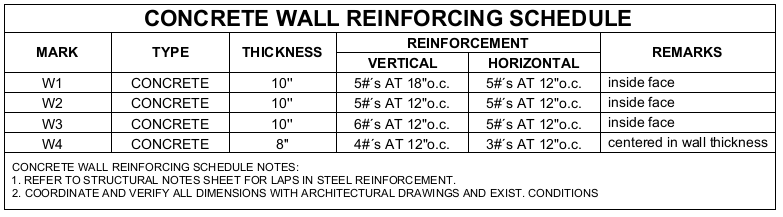
\includegraphics[width=\linewidth]{figures/concrete_wall_reinforcing_schedule.png}
    \caption{Concrete walls reinforcing schedule}\label{tb_concrete_wall_reinforcing_schedule}
\end{table}

\subsubsection{Wall types}
For analysis purposes we have considered the following wall types:

\begin{center}
  \begin{tabular}{|l|c|}
    \hline
    \textbf{Wall} & \textbf{Stem} \\
    & \textbf{height (m)} \\
    \hline
T1 & 3.15\\
T2 & 2.74\\
T3 & 3.53\\
T4 & 3.12\\
T5 & 2.51\\
T6 & 3.43\\
    \hline
  \end{tabular}
\end{center}

\subsubsection{Internal forces}
The envelope of internal forces envelope for each of the walls are given in tables \ref{tb_def_T1} to \ref{tb_def_T6}.

\begin{table}
\begin{center}
\begin{tabular}{|l|}
\hline
\multicolumn{1}{|c|}{\textsc{T1}}\\
\hline
\begin{tabular}{c|l}
\begin{minipage}{85mm}
\vspace{2mm}
\begin{center}
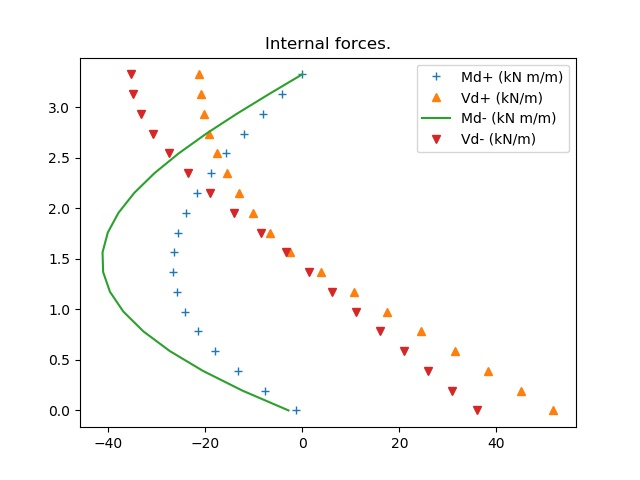
\includegraphics[width=80mm]{figures/T1}
\end{center}
\vspace{1pt}
\end{minipage} & 
\begin{tabular}{l}
\textsc{Wall geometry}\\
Stem top thickness: \\
$b_{top}= 0.25\ m$\\
Stem height: \\
$h_{stem}= 3.15\ m$\\
Stem bottom thickness: \\
$b_{bottom}= 0.25\ m$\\
Footing thickness: \\
$b_{footing}= 0.36\ m$\\
\end{tabular} \\
\end{tabular} \\
\hline
\begin{tabular}{llll}
\multicolumn{3}{c}{\textsc{Materials}}\\
  Concrete: C4000 &   Steel: A615G60 &   Concrete cover: 55 mm\\
\end{tabular} \\
\hline
\end{tabular}
\caption{Wall materials and dimensions T1} \label{tb_def_T1}
\end{center}
\end{table}

\begin{table}
\begin{center}
\begin{tabular}{|l|}
\hline
\multicolumn{1}{|c|}{\textsc{T2}}\\
\hline
\begin{tabular}{c|l}
\begin{minipage}{85mm}
\vspace{2mm}
\begin{center}
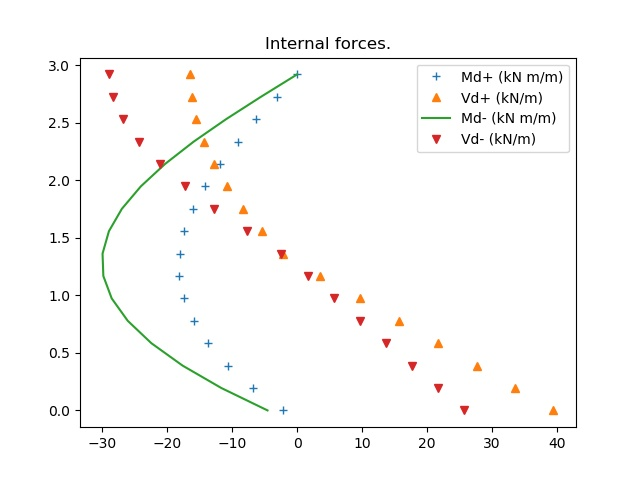
\includegraphics[width=80mm]{figures/T2}
\end{center}
\vspace{1pt}
\end{minipage} & 
\begin{tabular}{l}
\textsc{Wall geometry}\\
Stem top thickness: \\
$b_{top}= 0.25\ m$\\
Stem height: \\
$h_{stem}= 2.74\ m$\\
Stem bottom thickness: \\
$b_{bottom}= 0.25\ m$\\
Footing thickness: \\
$b_{footing}= 0.36\ m$\\
\end{tabular} \\
\end{tabular} \\
\hline
\begin{tabular}{llll}
\multicolumn{3}{c}{\textsc{Materials}}\\
  Concrete: C4000 &   Steel: A615G60 &   Concrete cover: 55 mm\\
\end{tabular} \\
\hline
\end{tabular}
\caption{Wall materials and dimensions T2} \label{tb_def_T2}
\end{center}
\end{table}


\begin{table}
\begin{center}
\begin{tabular}{|l|}
\hline
\multicolumn{1}{|c|}{\textsc{T3}}\\
\hline
\begin{tabular}{c|l}
\begin{minipage}{85mm}
\vspace{2mm}
\begin{center}
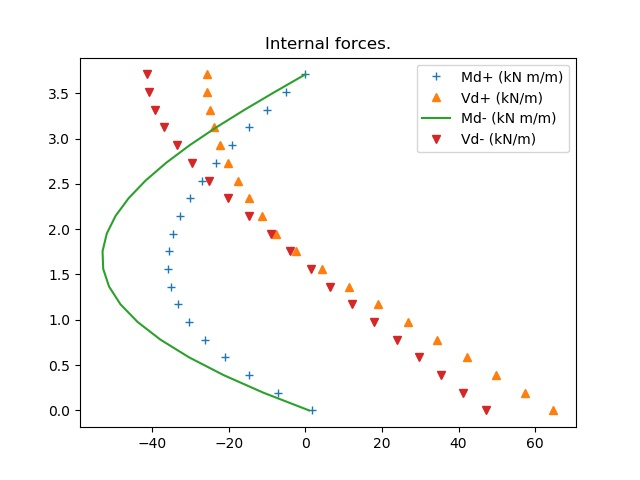
\includegraphics[width=80mm]{figures/T3}
\end{center}
\vspace{1pt}
\end{minipage} & 
\begin{tabular}{l}
\textsc{Wall geometry}\\
Stem top thickness: \\
$b_{top}= 0.25\ m$\\
Stem height: \\
$h_{stem}= 3.53\ m$\\
Stem bottom thickness: \\
$b_{bottom}= 0.25\ m$\\
Footing thickness: \\
$b_{footing}= 0.36\ m$\\
\end{tabular} \\
\end{tabular} \\
\hline
\begin{tabular}{llll}
\multicolumn{3}{c}{\textsc{Materials}}\\
  Concrete: C4000 &   Steel: A615G60 &   Concrete cover: 55 mm\\
\end{tabular} \\
\hline
\end{tabular}
\caption{Wall materials and dimensions T3} \label{tb_def_T3}
\end{center}
\end{table}



\begin{table}
\begin{center}
\begin{tabular}{|l|}
\hline
\multicolumn{1}{|c|}{\textsc{T4}}\\
\hline
\begin{tabular}{c|l}
\begin{minipage}{85mm}
\vspace{2mm}
\begin{center}
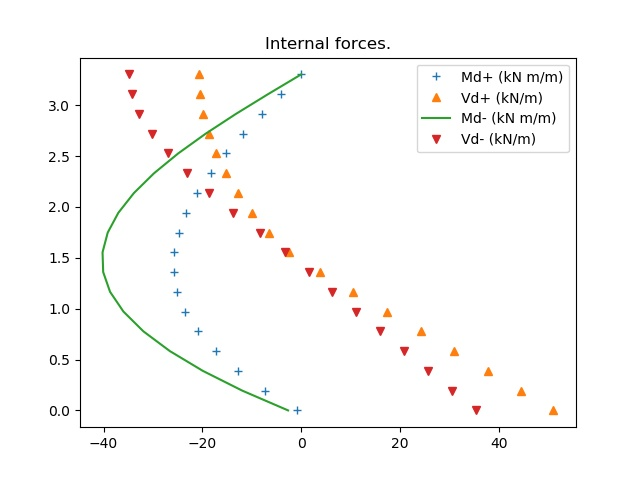
\includegraphics[width=80mm]{figures/T4}
\end{center}
\vspace{1pt}
\end{minipage} & 
\begin{tabular}{l}
\textsc{Wall geometry}\\
Stem top thickness: \\
$b_{top}= 0.25\ m$\\
Stem height: \\
$h_{stem}= 3.12\ m$\\
Stem bottom thickness: \\
$b_{bottom}= 0.25\ m$\\
Footing thickness: \\
$b_{footing}= 0.36\ m$\\
\end{tabular} \\
\end{tabular} \\
\hline
\begin{tabular}{llll}
\multicolumn{3}{c}{\textsc{Materials}}\\
  Concrete: C4000 &   Steel: A615G60 &   Concrete cover: 55 mm\\
\end{tabular} \\
\hline
\end{tabular}
\caption{Wall materials and dimensions T4} \label{tb_def_T4}
\end{center}
\end{table}

\begin{table}
\begin{center}
\begin{tabular}{|l|}
\hline
\multicolumn{1}{|c|}{\textsc{T5}}\\
\hline
\begin{tabular}{c|l}
\begin{minipage}{85mm}
\vspace{2mm}
\begin{center}
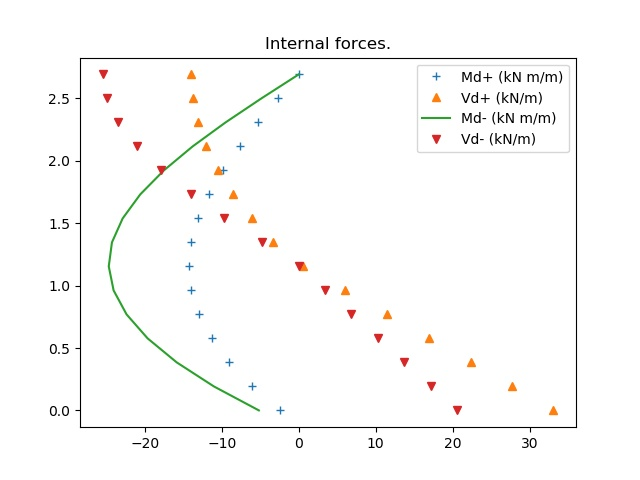
\includegraphics[width=80mm]{figures/T5}
\end{center}
\vspace{1pt}
\end{minipage} & 
\begin{tabular}{l}
\textsc{Wall geometry}\\
Stem top thickness: \\
$b_{top}= 0.25\ m$\\
Stem height: \\
$h_{stem}= 2.51\ m$\\
Stem bottom thickness: \\
$b_{bottom}= 0.25\ m$\\
Footing thickness: \\
$b_{footing}= 0.36\ m$\\
\end{tabular} \\
\end{tabular} \\
\hline
\begin{tabular}{llll}
\multicolumn{3}{c}{\textsc{Materials}}\\
  Concrete: C4000 &   Steel: A615G60 &   Concrete cover: 55 mm\\
\end{tabular} \\
\hline
\end{tabular}
\caption{Wall materials and dimensions T5} \label{tb_def_T5}
\end{center}
\end{table}


\begin{table}
\begin{center}
\begin{tabular}{|l|}
\hline
\multicolumn{1}{|c|}{\textsc{T6}}\\
\hline
\begin{tabular}{c|l}
\begin{minipage}{85mm}
\vspace{2mm}
\begin{center}
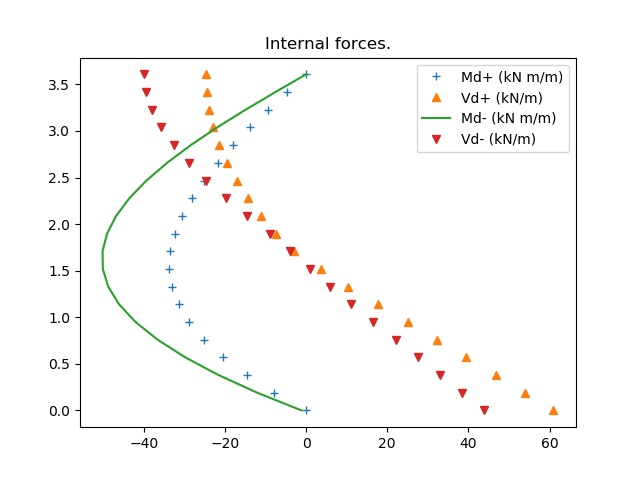
\includegraphics[width=80mm]{figures/T6}
\end{center}
\vspace{1pt}
\end{minipage} & 
\begin{tabular}{l}
\textsc{Wall geometry}\\
Stem top thickness: \\
$b_{top}= 0.25\ m$\\
Stem height: \\
$h_{stem}= 3.43\ m$\\
Stem bottom thickness: \\
$b_{bottom}= 0.25\ m$\\
Footing thickness: \\
$b_{footing}= 0.36\ m$\\
\end{tabular} \\
\end{tabular} \\
\hline
\begin{tabular}{llll}
\multicolumn{3}{c}{\textsc{Materials}}\\
  Concrete: C4000 &   Steel: A615G60 &   Concrete cover: 55 mm\\
\end{tabular} \\
\hline
\end{tabular}
\caption{Wall materials and dimensions T6} \label{tb_def_T6}
\end{center}
\end{table}

\subsubsection{Reinforcement checks}

\tablefirsthead{\hline
\multicolumn{1}{|c|}{\textsc{Wall vertical reinforcements}}\\\hline
}
\tablehead{\hline
\multicolumn{1}{|c|}{\textsc{wall vertical reinforcements (cont.)}}\\\hline
}
\tabletail{\hline \multicolumn{1}{|r|}{../..}\\\hline}
\tablelasttail{\hline}
\begin{center}
\begin{supertabular}{|l|}
\hline
\textbf{T1 wall. Inside stem reinforcement:}\\
  RC section dimensions; b= 1.00 m, h= 0.25 m\\
  diam: 16 mm, spacing: 300 mm  reinf. development L=0.34 m (22 diameters).\\
  area: As=   6.67 cm2/m areaMin:   4.56 cm2/m  F(As)= 1.46 OK!\\
  Bending check: Md=  40.09 kN m, MR=  41.36kN m  F(M)= 1.03 OK!\\
  Shear check: Vd=   7.61 kN,  VR= 199.37 kN  F(V)= 26.21 OK!\\
  %% Stress check: M=  40.09 kN m, $\sigma_s$= 263.03 MPa\\
  %%   $\sigma_{lim}$= 300.00 MPa  F($\sigma_s$)= 1.14 OK!\\
\hline
\textbf{T2 wall. Inside stem reinforcement:}\\
  RC section dimensions; b= 1.00 m, h= 0.25 m\\
  diam: 16 mm, spacing: 400 mm  reinf. development L=0.34 m (22 diameters).\\
  area: As=   5.00 cm2/m areaMin:   4.56 cm2/m  F(As)= 1.10 OK!\\
  Bending check: Md=  29.02 kN m, MR=  31.02kN m  F(M)= 1.07 OK!\\
  Shear check: Vd=   6.84 kN,  VR= 199.37 kN  F(V)= 29.15 OK!\\
  %% Stress check: M=  29.02 kN m, $\sigma_s$= 253.88 MPa\\
  %%   $\sigma_{lim}$= 300.00 MPa  F($\sigma_s$)= 1.18 OK!\\
\hline
\textbf{T3 wall. Inside stem reinforcement:}\\
  RC section dimensions; b= 1.00 m, h= 0.25 m\\
  diam: 19 mm, spacing: 300 mm  reinf. development L=0.61 m (32 diameters).\\
  area: As=   9.47 cm2/m areaMin:   4.56 cm2/m  F(As)= 2.08 OK!\\
  Bending check: Md=  51.88 kN m, MR=  58.26kN m  F(M)= 1.12 OK!\\
  Shear check: Vd=   7.98 kN,  VR= 199.37 kN  F(V)= 24.98 OK!\\
  %% Stress check: M=  51.88 kN m, $\sigma_s$= 239.75 MPa\\
  %%   $\sigma_{lim}$= 300.00 MPa  F($\sigma_s$)= 1.25 $\sim$ OK!\\
\hline
\textbf{T4 wall. Inside stem reinforcement:}\\
  RC section dimensions; b= 1.00 m, h= 0.25 m\\
  diam: 16 mm, spacing: 300 mm  reinf. development L=0.34 m (22 diameters).\\
  area: As=   6.67 cm2/m areaMin:   4.56 cm2/m  F(As)= 1.46 OK!\\
  Bending check: Md=  39.19 kN m, MR=  41.36kN m  F(M)= 1.06 OK!\\
  Shear check: Vd=   7.46 kN,  VR= 199.37 kN  F(V)= 26.73 OK!\\
  %% Stress check: M=  39.19 kN m, $\sigma_s$= 257.14 MPa\\
  %%   $\sigma_{lim}$= 300.00 MPa  F($\sigma_s$)= 1.17 OK!\\
\hline
\textbf{T5 wall. Inside stem reinforcement:}\\
  RC section dimensions; b= 1.00 m, h= 0.25 m\\
  diam: 16 mm, spacing: 400 mm  reinf. development L=0.34 m (22 diameters).\\
  area: As=   5.00 cm2/m areaMin:   4.56 cm2/m  F(As)= 1.10 OK!\\
  Bending check: Md=  23.62 kN m, MR=  31.02kN m  F(M)= 1.31 OK!\\
  Shear check: Vd=   6.42 kN,  VR= 199.37 kN  F(V)= 31.05 OK!\\
  %% Stress check: M=  23.62 kN m, $\sigma_s$= 206.69 MPa\\
  %%   $\sigma_{lim}$= 300.00 MPa  F($\sigma_s$)= 1.45 OK!\\
\hline
\textbf{T6 wall. Inside stem reinforcement:}\\
  RC section dimensions; b= 1.00 m, h= 0.25 m\\
  diam: 19 mm, spacing: 300 mm  reinf. development L=0.61 m (32 diameters).\\
  area: As=   9.47 cm2/m areaMin:   4.56 cm2/m  F(As)= 2.08 OK!\\
  Bending check: Md=  49.02 kN m, MR=  58.26kN m  F(M)= 1.19 OK!\\
  Shear check: Vd=   8.13 kN,  VR= 199.37 kN  F(V)= 24.54 OK!\\
  %% Stress check: M=  49.02 kN m, $\sigma_s$= 226.52 MPa\\
  %%   $\sigma_{lim}$= 300.00 MPa  F($\sigma_s$)= 1.32 OK!\\
\end{supertabular}
\end{center}

\tablefirsthead{\hline
\multicolumn{1}{|c|}{\textsc{Shear check}}\\\hline
}
\tablehead{\hline
\multicolumn{1}{|c|}{\textsc{shear check (cont.)}}\\\hline
}
\tabletail{\hline \multicolumn{1}{|r|}{../..}\\\hline}
\tablelasttail{\hline}
\begin{center}
\begin{supertabular}{|l|}
\textbf{T1 wall. Shear check:}\\
  Shear check: Vd=  42.99 kN,  VR= 199.37 kN  F(V)= 4.64 OK!\\
\hline
\textbf{T2 wall. Shear check:}\\
  Shear check: Vd=  31.78 kN,  VR= 199.37 kN  F(V)= 6.27 OK!\\
\hline
\textbf{T3 wall. Shear check:}\\
  Shear check: Vd=  55.00 kN,  VR= 199.37 kN  F(V)= 3.63 OK!\\
\hline
\textbf{T4 wall. Shear check:}\\
  Shear check: Vd=  42.35 kN,  VR= 199.37 kN  F(V)= 4.71 OK!\\
\hline
\textbf{T5 wall. Shear check:}\\
  Shear check: Vd=  26.03 kN,  VR= 199.37 kN  F(V)= 7.66 OK!\\
\hline
\textbf{T6 wall. Shear check:}\\
  Shear check: Vd=  51.43 kN,  VR= 199.37 kN  F(V)= 3.88 OK!\\
\end{supertabular}
\end{center}

\subsubsection{Wall foundations}
The results obtained for the verifications of the footing stability and the soil-bearing capacity. According to the geotechnical report the allowable soil bearing pressure is 3000 psf ($143.64\ kN/m^2$).
\begin{center}
\begin{tabular}{|l|c|c|c|}
\hline
\multicolumn{4}{|c|}{\textsc{wall foundation: T1}}\\
\hline
Verification:  & $F_{disp}$ & $F_{req}$ & Combination\\
\hline
Overturning:  & $\gg 1$ & 1.00 & EQ1609A\\
Sliding:  & 1.23 & 1.00 & EQ1609A\\
Adm. pressure:  & 1.09 & 1.00 & EQ1613B\\
\hline
\multicolumn{4}{|c|}{\textsc{wall foundation: T2}}\\
\hline
Verification:  & $F_{disp}$ & $F_{req}$ & Combination\\
\hline
Overturning:  & $\gg 1$ & 1.00 & EQ1613B\\
Sliding:  & 1.46 & 1.00 & EQ1609A\\
Adm. pressure:  & 1.13 & 1.00 & EQ1613B\\
\hline
\multicolumn{4}{|c|}{\textsc{wall foundattion: T3}}\\
\hline
Verification:  & $F_{disp}$ & $F_{req}$ & Combination\\
\hline
Overturning:  & $\gg 1$ & 1.00 & EQ1609A\\
Sliding:  & 1.13 & 1.00 & EQ1609A\\
Adm. pressure:  & 1.12 & 1.00 & EQ1613B\\
\hline
\multicolumn{4}{|c|}{\textsc{wall foundation: T4}}\\
\hline
Verification:  & $F_{disp}$ & $F_{req}$ & Combination\\
\hline
Overturning:  & $\gg 1$ & 1.00 & EQ1613B\\
Sliding:  & 1.45 & 1.00 & EQ1609A\\
Adm. pressure:  & 1.08 & 1.00 & EQ1613B\\
\hline
\multicolumn{4}{|c|}{\textsc{wall foundation: T5 }}\\
\hline
Verification:  & $F_{disp}$ & $F_{req}$ & Combination\\
\hline
Overturning:  & $\gg 1$ & 1.00 & EQ1613B\\
Sliding:  & 1.69 & 1.00 & EQ1609A\\
Adm. pressure:  & 1.22 & 1.00 & EQ1613B\\
\hline
\multicolumn{4}{|c|}{\textsc{wall foundation: T6}}\\
\hline
Verification:  & $F_{disp}$ & $F_{req}$ & Combination\\
\hline
Overturning:  & $\gg 1$ & 1.00 & EQ1609A\\
Sliding:  & 1.10 & 1.00 & EQ1609A\\
Adm. pressure:  & 1.03 & 1.00 & EQ1613B\\
\hline
\multicolumn{4}{|l|}{$F_{avail.}$: available security.}\\
\multicolumn{4}{|l|}{$F_{req}$: required security.}\\
\hline
\end{tabular}
\end{center}
